

In terms of when the order matching takes place, 
Double auction markets are generally divided into sealed-bid double 
auctions and continuous double auctions (CDA). In sealed-bid double 
auctions the orders are submitted only onces and then matched 
whereas in CDA the orders are matched with existing order book
as they come. Periodical double auction is an extension of sealed-bid 
double auction in which order submissions takes place in rounds. \citep*{Moc15} \\


In some implementations, such as \citet{God93}'s, a 
trade is formed only when a buyer and a seller each agree on 
the exact trade price but typically the crossing orders are matched 
automatically in a way that the trade price is still equal or better 
than the ask and bid prices. There are several algorithms for order 
match-ing. Some implementations try to match the orders as they come 
and put them to the orderbook only if they cannot be matched and some 
matches the orders at the end of a specified session. \\

The advantages of double auction markets are that they are typically more efficient compared to one sided auction. Only trades that are
Double auction markets treat both sides equally and are transparent but the method for price formation differs.\\



Zaraba & Itayose

There are two distinct models for centralized order matching:
call-market and continuous session market. The main distinction
is when the orders are to be matched: in call-market it happens
at the end of a trading period and in continuous session constantly
during the opening hours of the market. \citep{boer05} \citet{ASt05} 
used term \textit{Itayose method} for call-market and \textit{Zaraba method} for 
continuous session market and \citet{Moc15} used term periodic double auction
for describing call-market. Periodic double auction market can also be seen as 
an extension of sealed-bid auction in which 
Itayose method
is more common in artificial market settings but Zaraba method 
is more popular in real markets. 


According to , there are two distinct 
There are two common clearing methods in real world markets: 
Itayose and Zaraba methods. The most notable difference is 
when the settling process takes places. In Itayose markets 
orders are cumulated thorough a trading session and after 
then, clearing takes place. At the end of a session, orders 
are ordered according to their limit price and a price that 
maximizes the traded volume is chosen as the market price of 
the session. In Zaraba methods the clearing is an ongoing process. 
Each order is evaluated as they come whether they can be fulfilled 
or not with current state of the order book and in case they 
cannot be fulfilled they are put to the order book waiting 
for upcoming opposite orders. Kawamura et al. (??) found 
out with arti-ficial markets that Zaraba is able to fulfil 
more orders per trading session than Itay-ose but closing 
price is more volatile. I chose Zaraba method for matching 
mechanics in this thesis as it is closer to the mechanics 
used in western markets. This decision should also make 
the simulations more dynamic but opens up the possibility 
to leverage from the order book.






% Junk?
\citet{lob13} explained thorougly the price mechanics in continuous market. I 
further generalize their explanation to include also periodical auctions.
When clearing occurs, bid orders are matched with ask orders in a way that a 
trade forms between a bid with a price p\textsubscript{b} and an ask with a price 
p\textsubscript{a} where p\textsubscript{b} $\geq$ p\textsubscript{a}. No order
should be executed with a worse price than stated in the order. However, it is likely
that not all the bids that have higher price than the lowest ask and not all the asks that
have lower price than the highest bid in the market can be matched due to the asymmetricity 
of quantity per price level. Which of these orders gets executed and what price depends on 
the details of the underlying algorithm used in the market. Before going into this with more
detail, the problem is visually described for clarification.

A simple illustration of the order book evolution is presented
in the figure ~\ref{fig:lob_evo}: the order book receives two new bids in t, bids 1 and 2.
On t + 1, clearing occurs and the bid 2 is matched with one of the equal sized best ask orders.
Bid 1 is left in the order book and becomes the best bid order. As the order prices differ
between the bid 2 and the corresponding ask, it is not entirely obvious which price to pick
for the trade: bid's price, ask's price or the average. Especially in continuous markets,
the trade price is set according to the order that was in the order book already, in this
example the ask order. % Something about supply demand price matching etc.

\begin{figure}
    \begin{center}  
        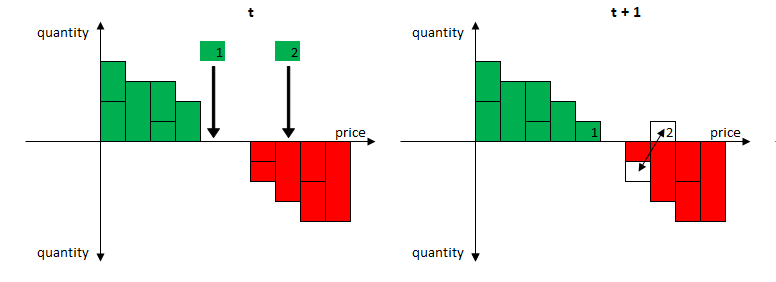
\includegraphics[width=15cm]{diagrams/lob_evolution.png}
        \caption{Evolution of a limit order book}
        \label{fig:lob_evo}
    \end{center}
\end{figure}

% Price formation in continuous settings
Price formation in continuous double auction is rather straight forward. Continuous
market do not allow clearable orders to stay in the limit order book thus the
candidates for trades can be narrowed down only to the opposing orders with better
or equal price than the newly arrived order. This is because the steps for 
clearing is conducted each time a new order arrives.



